\chapter{Progettazione Logica}
L'obiettivo della progettazione logica è quello di costruire uno schema logico in grado di descrivere in maniera corretta ed efficiente tutte le informazioni contenute nello schema E-R prodotto nella fase di progettazione concettuale.\\
Non si tratta di una semplice traduzione da un modello a un altro, in quanto, prima di passare allo schema logico, lo schema E-R va ristrutturato per soddisfare due esigenze: quella di semplificare la traduzione e quella di ottimizzare il progetto.\\
La semplificazione dello schema si rende necessaria perché non tutti i costrutti del modello E-R hanno una traduzione naturale nei modelli logici. Per esempio, mentre un'entità può essere facilmente rappresentata da una relazione del modello relazionale (avente gli stessi attributi dell'entità), per le generalizzazioni esistono varie alternative.\\
Inoltre, mentre la progettazione concettuale ha come obbiettivo la rappresentazione accurata e naturale dei dati d'interesse dal punto di vista del significato che hanno nell'applicazione, la progettazione logica costituisce la base per l'effettiva realizzazione dell'applicazione e deve tenere conto, per quanto possibile, delle sue prestazioni: questa necessità può portare a una ristrutturazione dello schema concettuale.



\section{Fasi della progettazione logica}
Le principali fasi della progettazione logica sono le seguenti:
    \begin{itemize}
        \item{\textbf{Ristrutturazione dello schema E-R}: è una fase indipendente dal modello logico scelto e si basa su criteri di ottimizzazione dello schema e di semplificazione della fase successiva.}
        \item{\textbf{Traduzione verso il modello logico}: fa riferimento a uno specifico modello logico (nel nostro caso il modello relazionale) e può includere un'ulteriore ottimizzazione che si basa sulle caratteristiche del modello logico stesso.}
    \end{itemize}
I dati in ingresso della prima fase sono lo schema concettuale prodotto nella fase precedente e il carico applicativo previsto, in termini di dimensione dei dati e caratteristiche delle operazioni.\\
Il risultato che si ottiene è uno schema E-R ristrutturato, che non è più uno schema concettuale nel senso stretto del termine, in quanto costituisce una rappresentazione dei dati che tiene conto degli aspetti realizzativi.\\\\
Questo schema e il modello logico scelto costituiscono i dati in ingresso della seconda fase, che produce lo schema logico della nostra base di dati.\\
In questa seconda fase è possibile effettuare verifiche della qualità dello schema ed eventuali ulteriori ottimizzazioni mediante tecniche basate sulle caratteristiche del modello logico.\\
La tecnica usata nell'ambito del modello relazionale è la \textbf{normalizzazione}.\\
Lo schema logico finale, i vincoli d'integrità definiti su di esso e la relativa documentazione costituiscono i prodotti finali della progettazione logica.



\section{Analisi delle prestazioni su schemi E-R}
Uno schema E-R può essere modificato per ottimizzare alcuni \textbf{indici di prestazione} del progetto. Facciamo riferimento ad indici di prestazione e non di prestazioni perché, in realtà, le prestazioni di una base dati non sono valutabili in maniera precisa in sede di progettazione logica, in quanto dipendenti anche da parametri fisici, dal sistema di gestione di basi di dati che verrà utilizzato e da altri fattori difficilmente prevedibili in questa fase.\\
È comunque possibile, facendo uso di alcune schematizzazioni, effettuare studi di massima dei due parametri che generalmente regolano le prestazioni dei sistemi software:  
    \begin{itemize}
        \item{\textbf{Costo di un'operazione}: viene valutato in termini di numero di occorrenze di entità e associazioni che mediamente vanno visitate per rispondere a un'operazione sulla base di dati.}
        \item{\textbf{Occupazione di memoria}: viene valutato in termini dello spazio di memoria (misurato, per esempio, in numero di byte) necessario per memorizzare i dati descritti dallo schema.}
    \end{itemize}
Per studiare questi parametri, abbiamo bisogno di conoscere (oltre allo schema) le seguenti informazioni:
    \begin{itemize}
        \item{\textbf{Volume dei dati}:
            \begin{itemize}
                \item{Numero di occorrenze di ogni entità e associazione dello schema}
                \item{Dimensioni di ciascun attributo}
            \end{itemize}}
        \item{\textbf{Caratteristiche delle operazioni}:
            \begin{itemize}
                \item{Tipo dell'operazione (interattiva o batch)}
                \item{Frequenza (numero medio di esecuzioni in un certo intervallo di tempo)}
                \item{Dati coinvolti (entità e/o associazioni)}
            \end{itemize}}
    \end{itemize}
Sebbene un'analisi delle prestazioni che fa riferimento a un numero ristretto di operazioni può sembrare riduttiva rispetto al reale carico della base di dati va notato che le operazioni sulle basi di dati seguono la cosiddetta regola \textbf{ottanta-venti}.\\
In base a questa regola, l'ottanta per cento del carico è generato dal venti per cento delle operazioni. Questo fatto ci consente di valutare adeguatamente il carico concetrandoci solo sulle operazioni principali previste.\\\\
Nella \textbf{tavola dei volumi} vengono riportati tutti i concetti dello schema (entità e associazioni) con il volume previsto a regime:
    \begin{table}\caption{Tavola dei volumi}
        \begin{center}\begin{tabular}{|c|c|c|} \hline
        \textbf{Concetto} & \textbf{Tipo} & \textbf{Volume} \\ \hline
        Impiegato & E & 2000 \\ \hline
        Afferenza & R & 1900 \\ \hline
        Dipartimento & E & 80 \\ \hline
        Sede & E & 10\\ \hline
        \end{tabular}\end{center}
    \end{table}
Il volume dei dati e le caratteristiche generali delle operazioni possono essere descritti facendo uso di tabelle, dette \textbf{tavole delle operazioni}, in cui vengono riportati, per ogni operazione, la frequenza prevista e un simbolo che indica se l'operazione è interattiva ($I$) oppure batch ($B$).
    \begin{table}\caption{Tavola delle operazioni}
        \begin{center}\begin{tabular}{|c|c|c|} \hline
        \textbf{Operazioni} & \textbf{Tipo} & \textbf{Frequenza} \\ \hline
        Op.1 & I & 50 al giorno \\ \hline
        Op.2 & I & 100 al giorno \\ \hline
        Op.3 & I & 10 al giorno \\ \hline
        Op.4 & B & 2 a settimana\\ \hline
        \end{tabular}\end{center}
    \end{table}
Nella tavola dei volumi, il numero delle occorrenze delle associazioni dipende da due parametri: il numero di occorrenze delle entità coinvolte nelle associazioni e il numero (medio) di partecipazioni di un'occorrenza di entità alle occorrenze di associazioni.\\
A sua volta, il secondo parametro dipende dalle cardinalità delle associazioni.\\\\ 
Per ogni operazione, possiamo inoltre descrivere graficamente i dati coinvolti con uno \textbf{schema di operazione} che consiste nel frammento dello schema E-R interessato dall'operazione, sul quale viene disegnato il \textit{cammino logico} da percorrere per accedere alle informazioni di interesse.\\
Una volta ottenute queste informazioni, possiamo fare una stima del costo di un'operazione sulla base di dati contando il numero di accessi alle occorrenze di entità e associazioni necessario per eseguire l'operazione.\\\\
Per esprimere le modalità di accesso alle informazioni utilizziamo la \textbf{tavola degli accessi}, che è nella forma:
    \begin{table}\caption{Tavola degli accessi}
        \begin{center}\begin{tabular}{|c|c|c|c|} \hline
        \textbf{Concetto} & \textbf{Costrutto} & \textbf{Accessi} & \textbf{Tipo} \\ \hline
        Impiegato & Entità & 1 & L \\ \hline
        Afferenza & Relazione & 1 & L \\ \hline
        Dipartimento & Entità & 1 & L \\ \hline
        Impiegato & Entità & 1 & L \\ \hline
        \end{tabular}\end{center}
    \end{table}
Nell'ultima colonna di questa tabella viene riportato il tipo di accesso: $L$ per accesso in lettura e $S$ per accesso in scrittura. Questa distinzione va fatta perché, generalmente, le operazioni di scrittura sono più onerose di quelle in lettura (in quanto devono essere eseguite in modo esclusivo e possono richiedere l'aggiornamento di \textbf{indici}, che sono strutture ausiliarie per l'accesso efficiente ai dati).



\section{Ristrutturazione di schemi E-R}
La fase di ristrutturazione di uno shcema E-R si può suddividere in una serie di passi da effettuare in sequenza:
    \begin{itemize}
        \item{\textbf{Analisi delle ridondanze}: si decide se eliminare o mantenere eventuali ridondanze presenti nello schema.}
        \item{\textbf{Eliminazione delle generalizzazioni}: tutte le generalizzazioni presenti nello schema vengono analizzate e sostituite da altri costrutti.}
        \item{\textbf{Partizionamento/accorpamento di entità e associazioni}: si decide se è opportuno partizionare concetti dello schema (entità e/o associazioni) in più concetti o, viceversa, accorpare concetti separati da un unico concetto.}
        \item{\textbf{Scelta degli identificatori principali}: si seleziona un identificatore per quelle entità che ne hanno più di uno.}
    \end{itemize}
    
\subsection{Analisi delle ridondanze}
Ricordiamo che una \textbf{ridondanza} in uno schema concettuale corrisponde alla presenza di un dato che può essere derivato (cioè ottenuto attraverso una serie di operazioni) da altri dati. In particolare, in uno schema E-R si possono presentare diversi tipi di ridondanza:
    \begin{itemize}
        \item{Attributi derivabili, occorrenza per occorrenza, da altri attributi della stessa entità (o associazione).}
        \item{Attributi derivabili da attributi di altre entità (o associazioni) di solito attraverso funzioni aggregative.}
        \item{Attributi derivabili da operazioni di conteggio di occorrenze. Si tratta, in effetti, di una variante del caso precedente, che viene però discusso separatamente perché molto frequente in pratica.}
        \item{Associazioni derivabili dalla composizione di altre associazioni in presenza di cicli. Notiamo che non sempre la presenza di un ciclo genera ridondanze!}
    \end{itemize}
La presenza di un dato derivato presenta un vantaggio e alcuni svantaggi. Il vantaggio è una riduzione degli accessi necessari per calcolare il dato derivato, gli svantaggi sono una maggiore occupazione di memoria (che è, comunque, spesso un costo trascurabile) e la necessità di effettuare operazioni aggiuntive per mantenere il dato derivato aggiornato.\\
La decisione di mantenere o eliminare una ridondanza va quindi presa confrontando costo di esecuzione delle operazioni che coinvolgono il dato ridondante e relativa occupazione di memoria, nei casi di presenza e assenza della ridondanza.

\subsection{Eliminazione delle generalizzazioni}
Dato che i sistemi tradizionali per la gestione delle basi di dati non consentono di rappresentare direttamente una generalizzazione, risulta spesso necessario trasformare questo costrutto in altri costrutti del modello E-R per i quali esiste invece una implementazione naturale: le entità e le associazioni.
     \begin{figure}
        \centering
        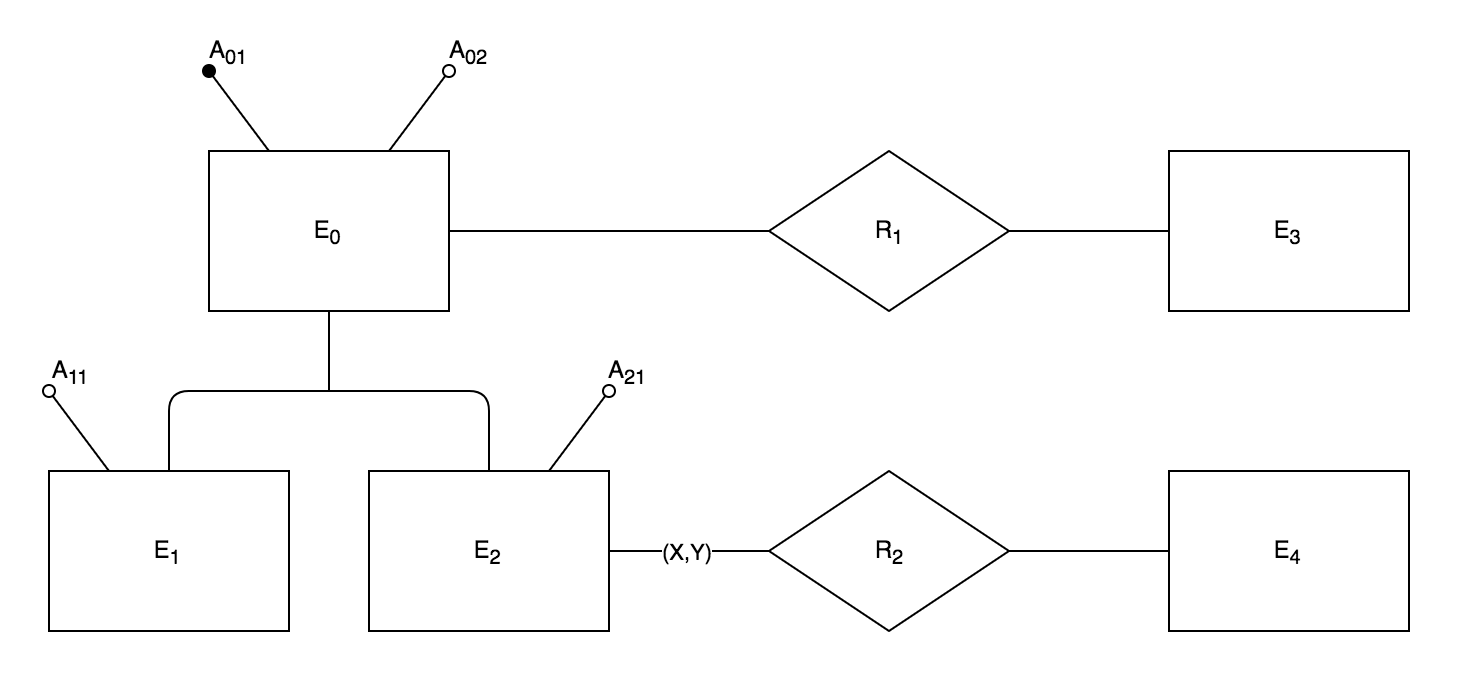
\includegraphics[scale=0.6]{15/img0}
        \caption{Generalizzazione: esempio}
    \end{figure}\\\\
Per rappresentare una generalizzazione mediante entità e associazioni abbiamo essenzialmente tre alternative possibili, che si eseguono attraverso le seguenti ristrutturazioni:
    \begin{enumerate}
        \item{\textbf{Accorpamento delle figlie della generalizzazione nel genitore.}\\
        Le entità $E_1$ ed $E_2$ vengono eliminate e le loro proprietà (attributi e partecipazioni ad associazioni e generalizzazioni) vengono aggiunte all'entità genitore $E_0$.\\
        A tale entità viene aggiunto un ulteriore attributo che serve a descrivere il "tipo" di una occorrenza di $E_0$, cioè se tale occorrenza apparteneva a $E_1$ oppure a $E_2$ o, nel caso di generalizzazione non totale, a nessuna di esse.
            \begin{figure}[h!]
                \centering
                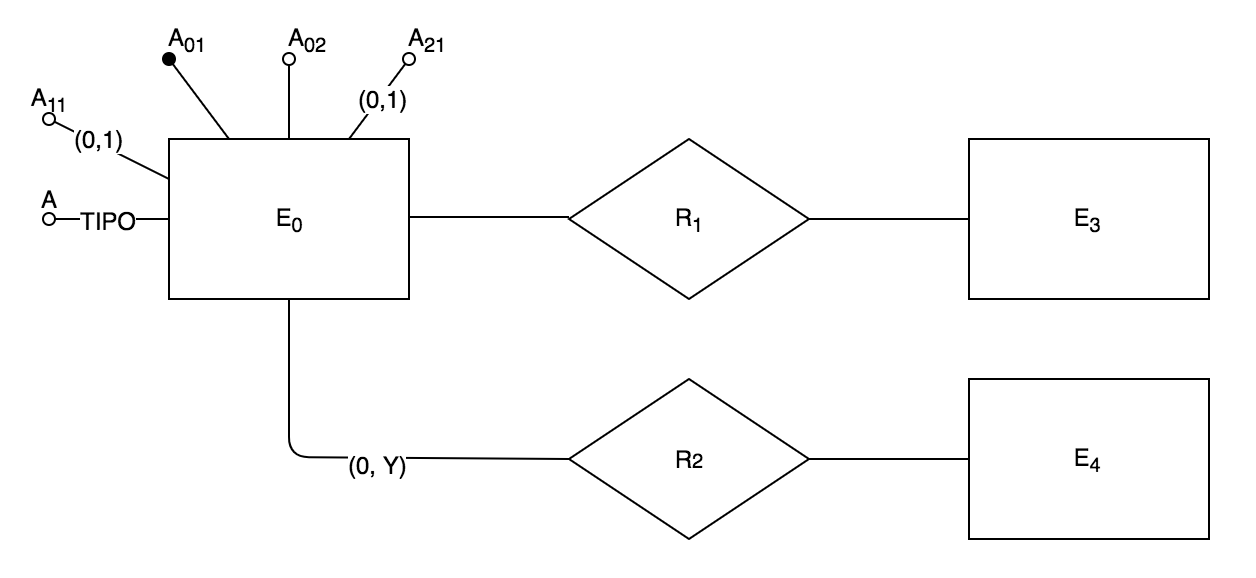
\includegraphics[scale=0.6]{15/img1}
                \caption{Ristrutturazione n.1}
            \end{figure}\\\\}
        \item{\textbf{Accorpamento del genitore della generalizzazione nelle figlie.}\\
        L'entità genitore $E_0$ viene eliminata e, per la proprietà dell'ereditarietà i suoi attributi, il suo identificatore e le relazioni a cui tale entità partecipava, vengono aggiunti alle entità figlie $E_1$ ed $E_2$.\\
        Le relazioni $R_{11}$ e $R_{12}$ rappresentano rispettivamente la restrizione della relazione $R_1$ sulle occorrenze delle entità $E_1$ ed $E_2$.
            \begin{figure}[h!]
                \centering
                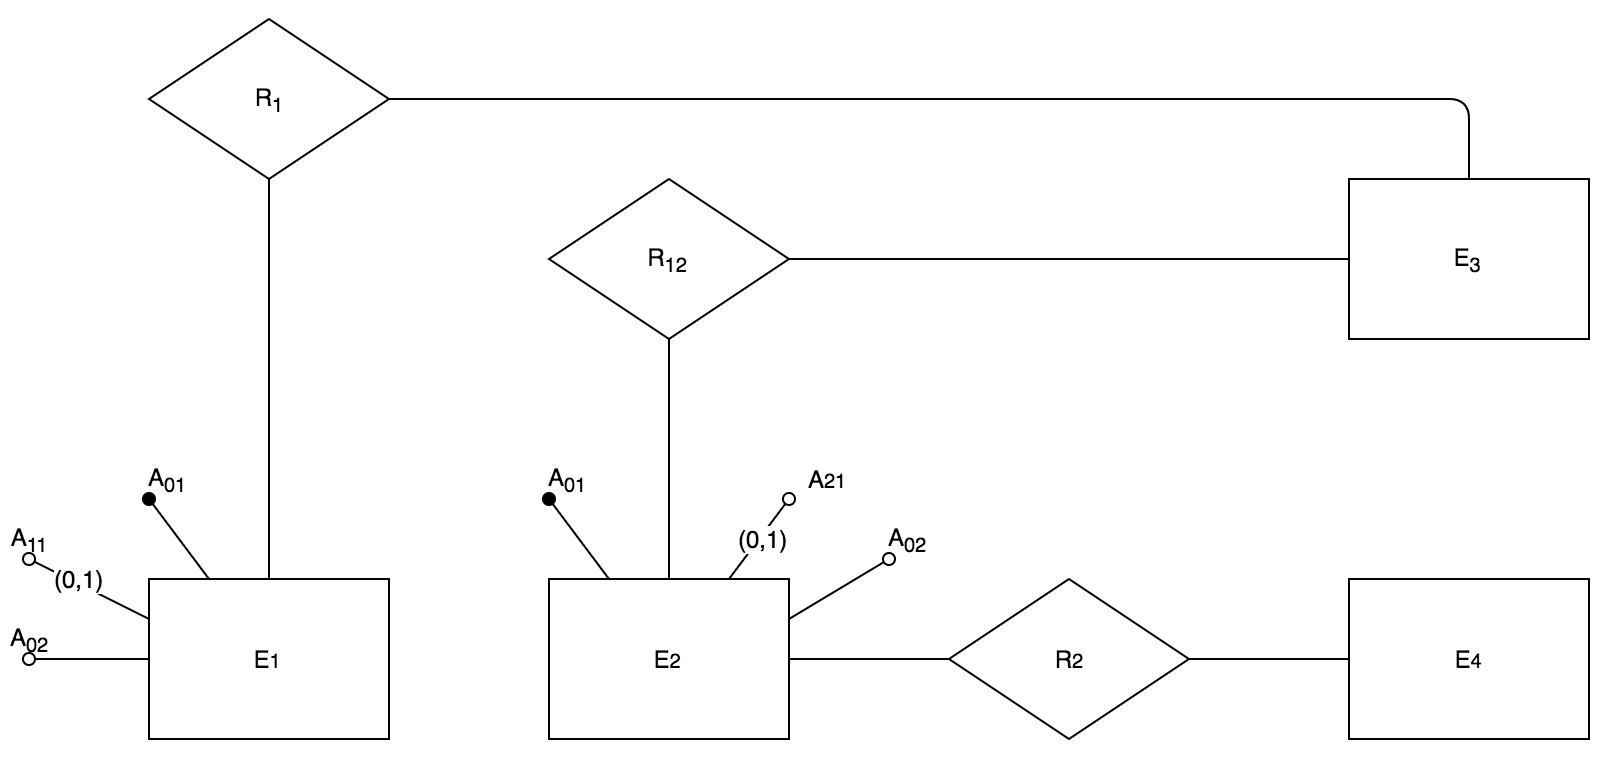
\includegraphics[scale=0.5]{15/img2}
                \caption{Ristrutturazione n.2}
            \end{figure}\\\\}
        \item{\textbf{Sostituzione della generalizzazione con associazioni.}\\
        La generalizzazione si trasforma in due associazioni uno a uno, che legano rispettivamente l'entità genitore con le entità figlie $E_1$ ed $E_2$. Non ci sono trasferimenti di attributi o associazioni e le entità $E_1$ ed $E_2$ sono identificate esternamente dall'entità $E_0$.\\
        Nello schema ottenuto vanno aggiunti, però, dei vincoli: ogni occorrenza di $E_0$ non può partecipare contemporaneamente a $R_{G1}$ e $R_{G2}$; inoltre, se la generalizzazione è totale, ogni occorrenza di $E_0$ deve partecipare o a un'occorrenza di $R_{G1}$ oppure a un'occorrenza di $R_{G2}$.
            \begin{figure}[h!]
                \centering
                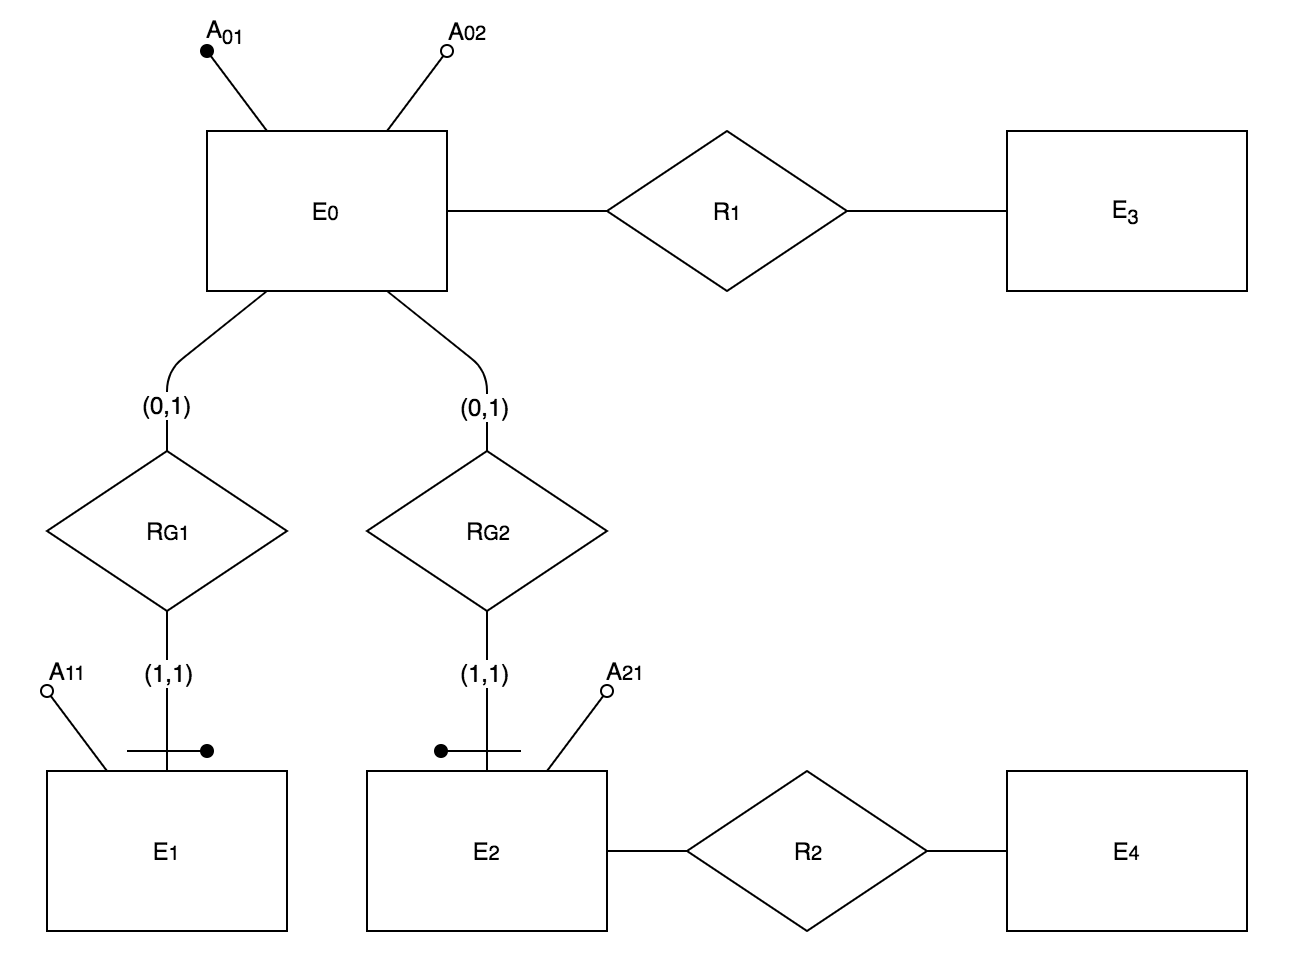
\includegraphics[scale=0.6]{15/img3}
                \caption{Ristrutturazione n.3}
            \end{figure}\\\\}
    \end{enumerate}
La scelta fra le varie alternative può essere fatta in maniera analoga a quanto fatto per i dati derivati, considerando vantaggi e svantaggi di ognuna delle scelte possibili relativamente all'occupazione di memoria e al costo delle operazioni coinvolte.\\
È comunque possibile stabilire alcune regole di carattere generale:
    \begin{enumerate}
        \item{\textbf{Alternativa n. 1}: conveniente quando le operazioni non fanno molta distinzione tra le occorrenze e gli attributi di $E_0$, $E_1$ ed $E_2$.\\
        In questo caso, infatti, anche se abbiamo uno spreco di memoria per la presenza di valori nulli, la scelta ci assicura un numero minore di accessi rispetto alle altre, nelle quali le occorrenze e gli attributi sono distribuiti tra le varie entità.}
        \item{\textbf{Alternativa n. 2}: possibile solo se la generalizzazione è totale, altrimenti le occorrenze di $E_0$ che non sono occorrenze né di $E_1$ né di $E_2$ non sarebbero rappresentate.\\
        È conveniente quando non ci sono operazioni che si riferiscono solo ad occorrenze di $E_1$ oppure di $E_2$, e dunque fanno delle distinzioni tra tali entità.\\
        In questo caso abbiamo un risparmio di memoria rispetto all'alternativa n.1 perché, in linea di principio, gli attributi non assumono mai valori nulli. Inoltre, c'è una riduzione degli accessi rispetto all'alternativa n.3 perché non si deve visitare $E_0$ per accedere ad alcuni attributi di $E_1$ ed $E_2$.}
        \item{\textbf{Alternativa n. 3}: conveniente quando la generalizzazione non è totale (sebbene ciò non sia necessario) e ci sono operazioni che si riferiscono solo a occorrenze di $E_1$ ($E_2$) oppure di $E_0$, e dunque fanno delle distinzioni tra entità figlia ed entità genitore.\\
        In questo caso abbiamo un risparmio di memoria rispetto all'alternativa n.1, per l'assenza di valori nulli, ma c'è un incremento degli accessi per mantenere la consistenza delle occorrenze rispetto ai vincoli introdotti.}
    \end{enumerate}
La ristrutturazione delle generalizzazioni è un tipico caso per il quale il semplice conteggio delle istanze e degli accessi non è sempre sufficiente per scegliere la migliore alternativa possibile.\\
Infatti, in base a quanto abbiamo detto, sembra che l'alternativa n.3 non convenga quasi mai perché richiede molti più accessi a occorrenze delle altre per eseguire le operazioni sui dati. Questa ristrutturazione, però, ha il grosso vantaggio di generare entità con pochi attributi. Come vedremo in seguito, questo si traduce a livello pratico, in strutture logiche di piccole dimensioni per le quali un accesso fisico permette di recuperare molti dati (tuple) in una sola volta.\\
In alcuni casi, quindi, va effettuata un'analisi più fine, che tiene conto di altri fattori quali le dimensioni dei domini degli attributi e la quantità di dati che è possibile recuperare con una sola operazione di accesso a memoria secondaria. 
    
\subsection{Partizionamento/accorpamento di concetti}
Entità e associazioni in uno schema E-R possono essere partizionati o accorpati per garantire una maggiore efficienza delle operazioni in base al seguente principio: gli accessi si riducono separando attributi di uno stesso concetto a cui accediamo attraverso operazioni diverse e raggruppando attributi di concetti diversi a cui accediamo attraverso medesime operazioni. Le stesse tecniche discusse per l'analisi delle generalizzazioni possono essere usate per prendere decisioni di questo tipo.\\\\
È importante notare che, in molti casi, i problemi di partizionamento/accorpamento possono essere rinviati alla fase di progettazione fisica.
\subsubsection{Partizionamenti di entità}
Esistono sostanzialmente due tipi di partizionamenti di entità:
    \begin{itemize}
        \item{\textbf{Partizionamenti verticali}: il concetto viene suddiviso operando sui suoi atttributi.\\
        I partizionamenti verticali generano entità con pochi attributi che possono essere tradotte in strutture logiche sulle quali, con un solo accesso, è possibile recuperare molti dati.}
        \item{\textbf{Partizionamenti orizzontali}: la suddivisione avviene sulle occorrenze dell'entità.\\
        Questo tipo di partizionamenti hanno un effetto collaterale: quello di dover duplicare tutte le associazioni a cui l'entità originaria partecipa. Questo fenomeno può avere delle ripercussioni negative sulle prestazioni del sistema.}
    \end{itemize}
Come per le generalizzazioni, anche in questo caso il semplce conteggio delle occorrenze e degli accessi, non è sempre sufficiente per scegliere la migliore alternativa possibile.
\subsubsection{Eliminazione di attributi multivalore}
Questa ristrutturazione si rende necessaria perché, come per le generalizzazioni, il modello relazionale non permette di rappresentare in maniera diretta questo tipo di attributo.\\
Per eliminare un attributo che ha cardinalità $(1,N)$, partizioniamo l'entità che lo contiene in due entità, tra loro legate da una nuova relazione.
    \begin{figure}
        \centering
        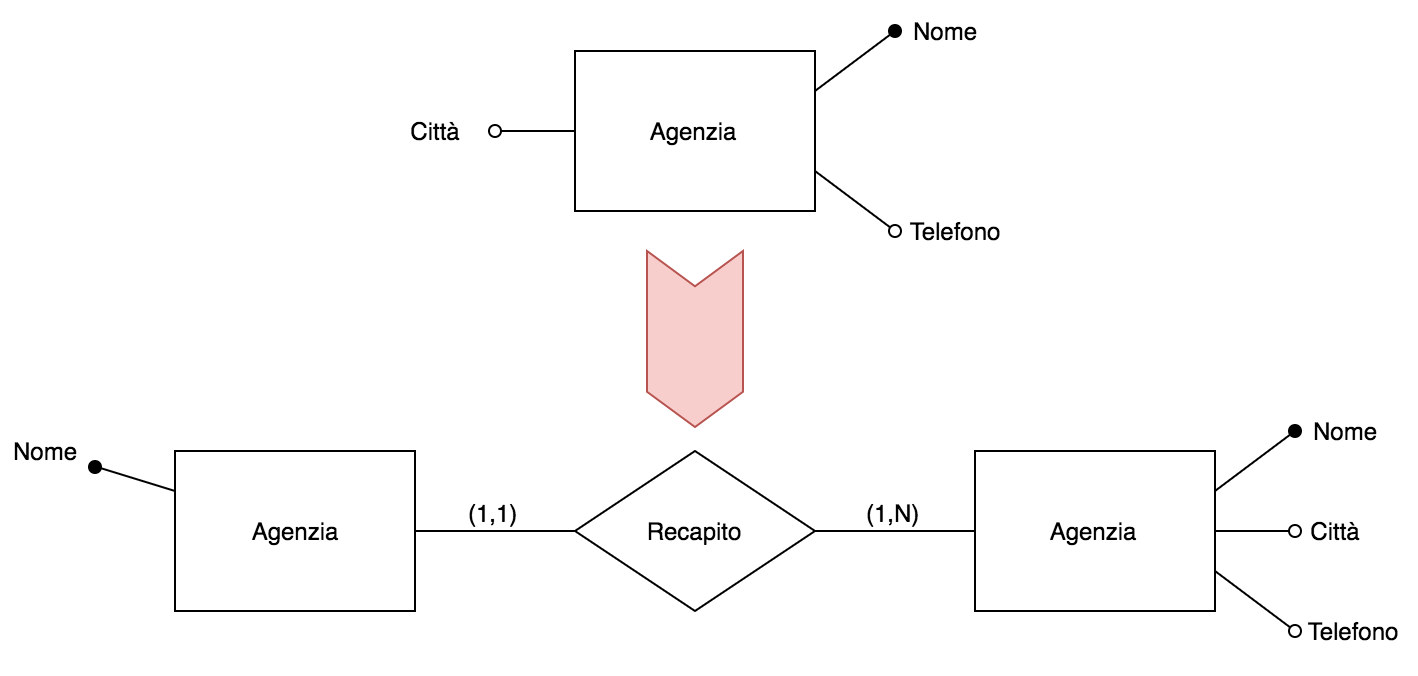
\includegraphics[scale = 0.6]{15/img4}
        \caption{Eliminazione di attributi multivalore}
    \end{figure}\\\\
\subsubsection{Accorpamento di entità}
L'accorpamento è l'operazione inversa del partizionamento.\\
Immaginiamo di avere una relazione $R$ tra due entità $E_1$ ed $E_2$. Nel caso in cui le operazioni sull'entità $E_1$ richiedano sempre i dati relativi ad $E_2$, vogliamo risparmiare gli accessi necessari per risalire a questi dati attraverso $R$. Per farlo, aggiungiamo gli attributi di $E_2$ ad $E_1$, ed eliminiamo $E_2$.\\
Un effetto collaterale di questa ristrutturazione è la possibile presenza di valori nulli causate dalla partecipazione opzionale dell'entità $E_1$ alla relazione $R$.\\
In genere, gli accorpamenti vengono effettuati su associazioni di tipo uno a uno, raramente su relazioni uno a molti e quasi mai su relazioni molti a molti. Questo perché gli accorpamenti di entità legate da un'associazione uno a molti o molti a molti generano ridondanze. In particolare, si possono presentare ridondanze su attributi non chiave dell'entità che partecipava all'associazione originaria con cardinalità massima pari a $N$.\\
La presenza di ridondanze può comunque essere discussa efficacemente attraverso la tecnica della \textbf{normalizzazione}.
\subsubsection{Altri tipi di partizionamento/accorpamento}
I discorsi fatti finora sul partizionamento/accorpamento possono essere estesi alle associazioni. In alcuni casi, infatti, può essere conveniente decomporre un'associazione tra due entità in due (o più) associazioni tra le medesime entità, per separare occorrenze dell'associazione originarie a cui effettuiamo l'accesso sempre separatamente o, viceversa, accorpare due (o più) associazioni tra le medesime entità (che si riferiscono a due aspetti dello stesso concetto) in un'unica associazione, quando accediamo alle relative occorrenze vengono sempre comtemporaneamente.


\subsection{Scelta degli identificatori principali}
La scelta degli identificatori principali è essenziale nelle traduzioni verso il modello relazionale perché in questo modello le chiavi vengono utilizzate per stabilire legami tra dati in relazioni diverse.\\
Inoltre, i sistemi di gestione di basi di dati richiedono generalmente di specificare una \textbf{chiave primaria} sulla quale vengono costruite automaticamente delle strutture ausiliarie, dette \textbf{indici}, per il reperimento efficiente di dati.\\
Quindi, nei casi in cui esistono entità per le quali sono stati specificati più identificatori, bisogna decidere quale di questi identificatori verrà utilizzato come chiave primaria.\\\\
I criteri di decisione per effettuare questa scelta sono i seguenti:
    \begin{itemize}
        \item{Gli attributi con valori nulli non possono costituire identificatori principali. Tali attributi, infatti, non garantiscono l'accesso a tutte le occorrenze dell'entità corrispondente.}
        \item{Un identificatore composto da uno o da pochi attributi è da preferire a identificatori costituiti da molti attributi. Questo garantisce che le strutture ausiliarie create per accedere ai dati (gli indici) siano di dimensioni ridotte, permette un risparmio di memoria nella realizzazione dei legami logici tra le varie relazioni e facilità le operazioni di join.}
        \item{Per le stesse motivazioni esposte al punto precedente, un identificatore interno è da preferire a un identificatore esterno, che magari coinvolge diverse entità.\\
        Infatti, gli identificatori esterni vengono tradotti in chiavi che includono gli identificatori delle entità coinvolte nell'identificazione esterna: chiaramente in questa maniera si possono generare chiavi con molti attributi.}
        \item{Un identificatore che viene utilizzato da molte operazioni per accedere alle occorrenze di un'entità è da preferire rispetto agli altri.\\
        In questa maniera tali operazioni possono essere eseguite efficientemente perché possono trarre vantaggio dagli indici creati automaticamente dal DBMS.}
    \end{itemize}
A questo punto, se nessuno degli identificatori candidati soddisfa tali requisiti, è possibile pensare di introdurre un ulteriore attributo all'entità: questo attributo conterrà valori speciali (detti \textbf{codici}) generati appositamente per identificare le occorrenze delle entità.\\
È comunque consigliabile tenere traccia, in questa fase, anche degli identificatori non selezionati come principali ma che vengono utilizzati da qualche operazione per accedere ai dati. Infatti, per questi identificatori è possibile definire, in sede di progettazione fisica, degli \textbf{indici secondari}. Gli indici secondari consentono l'accesso efficiente ai dati e possono essere usati in alternativa agli indici definiti automaticamente sugli identificatori principali. 

\section{Traduzione verso il modello relazionale}
La seconda fase della progettazione logica corrisponde a una traduzione tra modelli di dati diversi: a partire da uno schema E-R ristrutturato si costruisce uno \textbf{schema logico equivalente}, in grado cioè di rappresentare le medesime informazioni.\\
Coerentemente con quanto già detto, facciamo riferimento a una versione semplificata del modello E-R, che non contiene generalizzazioni e attributi multivalore, e nella quale ogni entità ha un solo identificatore. 

\subsection{Entità e associazioni molti a molti}
Consideriamo il seguente schema:
    \begin{figure}[h!]
        \centering
        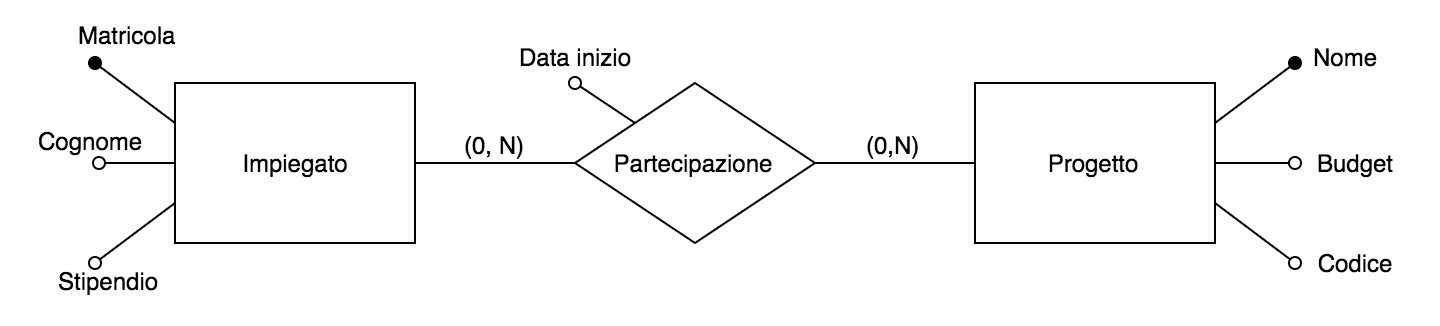
\includegraphics[scale = 0.5]{15/img5}
        \caption{Relazione molti a molti}
    \end{figure}\\\\
La sua traduzione naturale nel modello relazionale prevede:
    \begin{itemize}
        \item{Per ogni entità, una relazione con lo stesso nome avente per attributi i medesimi attributi dell'entità e per chiave il suo identificatore.}
        \item{Per l'associazione, una relazione con lo stesso nome avente per attributi gli attributi dell'associazione e gli identificatori delle entità coinvolte; tali identificatori formano la chiave della relazione.}
    \end{itemize}
Se gli attributi originali di entità o associazioni sono opzionali, i corrispondenti attributi di relazione possono assumere valori nulli.\\
Lo schema relazionale che otteniamo è, quindi, il seguente:
    \begin{equation}\begin{aligned}
        IMPIEGATO(\underline{Matricola}, Cognome, Stipendio)\\
        PROGETTO(\underline{Codice}, Nome, Budget)\\
        PARTECIPAZIONE(\underline{Matricola, Codice}, DataInizio)
    \end{aligned}\end{equation}
Per lo schema ottenuto esistono due vincoli d'integrità referenziale tra gli attributi $Matricola$ e $Codice$ di $PARTECIPAZIONE$ e gli omonimi attributi delle entità $IMPIEGATO$ e $PROGETTO$.\\\\
Possiamo, ovviamente effettuare delle ridenominazioni per rendere lo schema più leggibile, e siamo obbligati a farlo quando abbiamo a che fare con una relazione ricorsiva, come la seguente:
    \begin{figure}[h!]
        \centering
        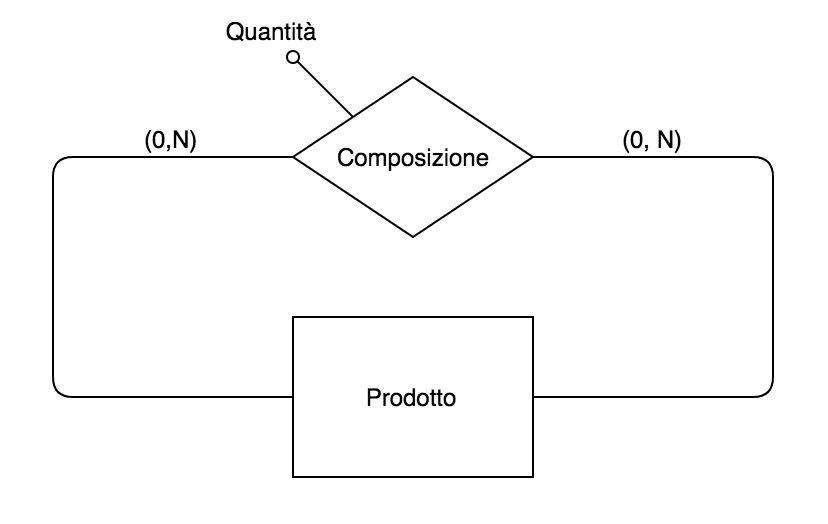
\includegraphics[scale = 0.5]{15/img6}
        \caption{Relazione ricorsiva}
    \end{figure}\\\\
Questo schema si traduce nelle due relazioni
    \begin{equation}\begin{aligned}
        PRODOTTO(\underline{Codice}, Nome, Costo)\\
        COMPOSIZIONE(\underline{Composto, Componente}, Quantita)
    \end{aligned}\end{equation}
In questo schema entrambi gli attributi $Composto$ e $Componente$ contengono codici di prodotti: il primo dei due ha il secondo come componente.\\
Esiste, quindi, un vincolo d'integrità referenziale tra questi attributi e l'attributo $Codice$ della relazione $PRODOTTO$.\\\\
Le associazioni con più di due entità  partecipanti si traducono in maniera analoga a quanto detto per le associazioni binarie.\\
Per esempio, consideriamo il seguente schema:
    \begin{figure}[h!]
        \centering
        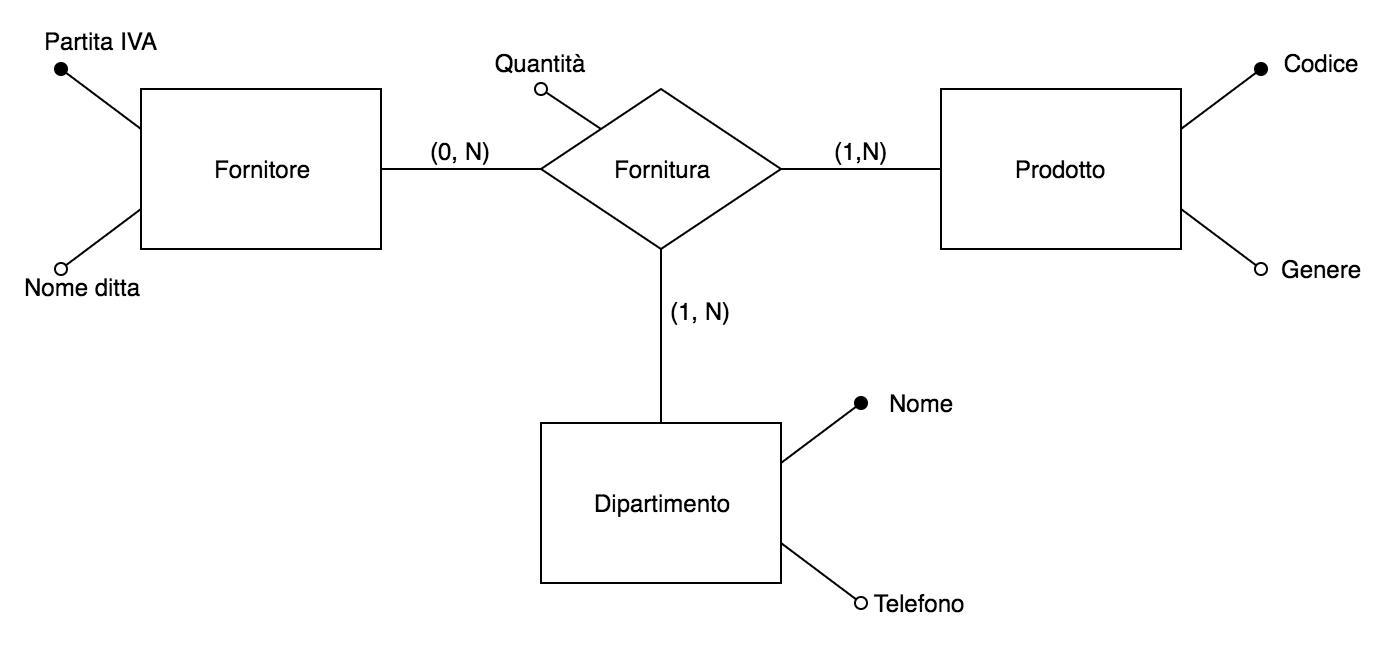
\includegraphics[scale = 0.5]{15/img7}
        \caption{Relazione ternaria}
    \end{figure}\\\\
Questo schema si traduce nelle seguenti relazioni:
    \begin{equation}\begin{aligned}
        FORNITORE(\underline{PartitaIVA}, NomeDitta)\\
        PRODOTTO(\underline{Codice, Genere})\\
        DIPARTIMENTO(\underline{Nome}, Telefono)\\
        FORNITURA(\underline{Fornitore, Prodotto, Dipartimento}, Quantita)
    \end{aligned}\end{equation}
Per lo schema così ottenuto esistono i vincoli d'integrità referenziale tra gli attributi $Fornitore$, $Prodotto$ e $Dipartimento$ della relazione $FORNITURA$ e, rispettivamente, l'attributo $PartitaIVA$ della relazione $FORNITORE$, l'attributo $Codice$ della relazione $PRODOTTO$ e l'attributo $Nome$ della relazione $DIPARTIMENTO$.\\\\
In quest'ultimo tipo di traduzione è necessario prestare attenzione ad alcuni casi particolari nei quali l'insieme delle chiavi delle relazioni che rappresentano le entità coinvolte costituisce in realtà una \textbf{superchiave} ridondante della relazione che rappresenta l'associazione dello schema E-R (esiste cioè un suo sottoinsieme proprio che è una chiave).\\
Questo potrebbe accadere se, per esempio, nel caso della relazione ternaria appena vista, ci fosse un solo fornitore che fornisce un certo prodotto a un dipartimento.\\
Si noti che le cardinalità sono ancora valide, perché tale fornitore può fornire diversi prodotti a questo o altri dipartimenti. In questo caso la chiave della relazione $FORNITURA$ sarebbe costituita dai soli attributi $Prodotto$ e $Dipartimento$, perché dato un prodotto e un dipartimento, il fornitore è univocamente determinato. 

\subsection{Associazioni uno a molti}
Consideriamo il seguente schema:
    \begin{figure}[h!]
        \centering
        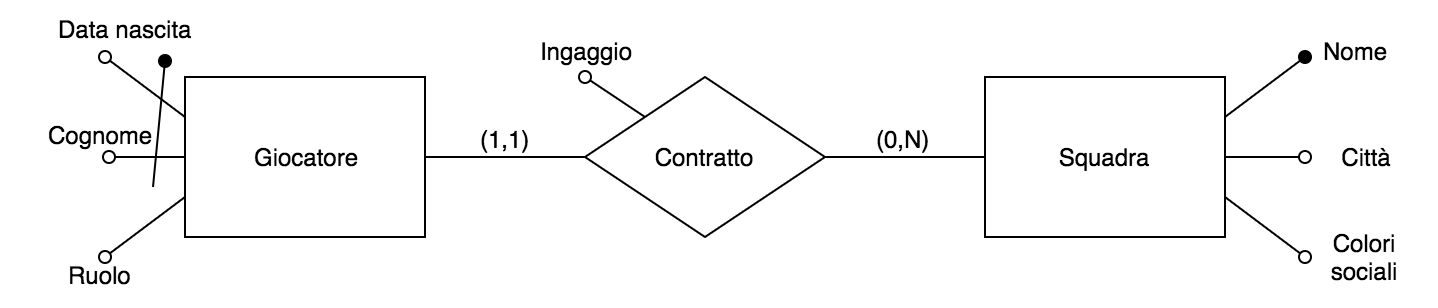
\includegraphics[scale = 0.5]{15/img8}
        \caption{Relazione uno a molti}
    \end{figure}\\\\
Secondo la regola vista per le associazioni molti a molti, la traduzione di questo schema dovrebbe essere la seguente: 
    \begin{equation}\begin{aligned}
        GIOCATORE(\underline{Cognome, DataNascita}, Ruolo)\\
        SQUADRA(\underline{Nome}, Citta, ColoriSociali)\\
        CONTRATTO(\underline{Giocatore, DataNascitaGiocatore}, NomeSquadra, Ingaggio)
    \end{aligned}\end{equation}
Notiamo che nella relazione $CONTRATTO$ la chiave è costituita solo dall'identificatore di $GIOCATORE$ perché le cardinalità indicano che ogni giocatore ha un contratto con una sola squadra.\\
A questo punto le relazioni $GIOCATORE$ e $CONTRATTO$ hanno ancora la stessa chiave ed è ancora possibile fonderle in un'unica relazione (perché esiste una corrispondenza biunivoca tra le rispettive occorrenze). È quindi preferibile la traduzion che segue:
    \begin{equation}\begin{aligned}
        GIOCATORE(\underline{Cognome, DataNascita}, Ruolo, NomeSquadra, Ingaggio)\\
        SQUADRA(\underline{Nome}, Citta, ColoriSociali)
    \end{aligned}\end{equation}
In questo schema, ovviamente, esiste il vincolo d'integrità referenziale tra l'attributo $NomeSquadra$ della relazione $GIOCATORE$ e l'attributo $Nome$ della relazione $SQUADRA$.\\\\
Le associazioni $n$-arie sono quasi sempre molti a molti. Nel caso in cui un'entità partecipi a una relazione ternaria con cardinalità massima pari a uno, la traduzione dell'associazione viene fatta in modo analogo a un'associazione binaria tra le altre entità.\\
L'entità che partecipa alla relazione ternaria con cardinalità massima pari a uno, viene infatti tradotta in una relazione che contiene anche gli identificatori delle altre entità coinvolte nell'associazione (più eventuali attributi dell'associazione stessa) e non è più necessario rappresentare esplicitamente l'associazione di partenza.\\
Consideriamo, per esempio, il seguente schema:
    \begin{figure}[h!]
        \centering
        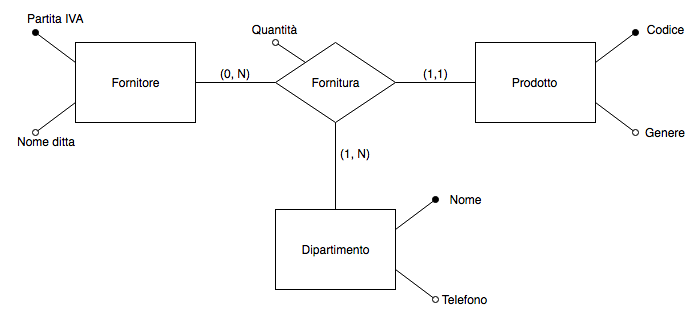
\includegraphics[scale = 0.5]{15/img8b}
        \caption{Relazione uno a molti}
    \end{figure}\\\\
Lo schema si traduce nelle seguenti relazioni:
    \begin{equation}\begin{aligned}
        FORNITORE(\underline{PartitaIVA}, NomeDitta)\\
        DIPARTIMENTO(\underline{Nome}, Telefono)\\
        PRODOTTO(\underline{Codice}, Genere, Fornitore, Dipartimento, Quantita)
    \end{aligned}\end{equation}
In tale schema relazionale esistono i vincoli d'integrità referenziale tra l'attributo $Fornitore$ della relazione $PRODOTTO$ e l'attributo $PartitaIVA$ della relazione $FORNITORE$ e tra l'attributo $Dipartimento$ della relazione $PRODOTTO$ e l'attributo $Nome$ della relazione $DIPARTIMENTO$.    

\subsection{Entità con identificatore esterno}
Le entità con identificatori esterni danno luogo a relazioni con chiavi che includono gli identificatori delle entità "identificanti".\\
Consideriamo il seguente schema:
    \begin{figure}[h!]
        \centering
        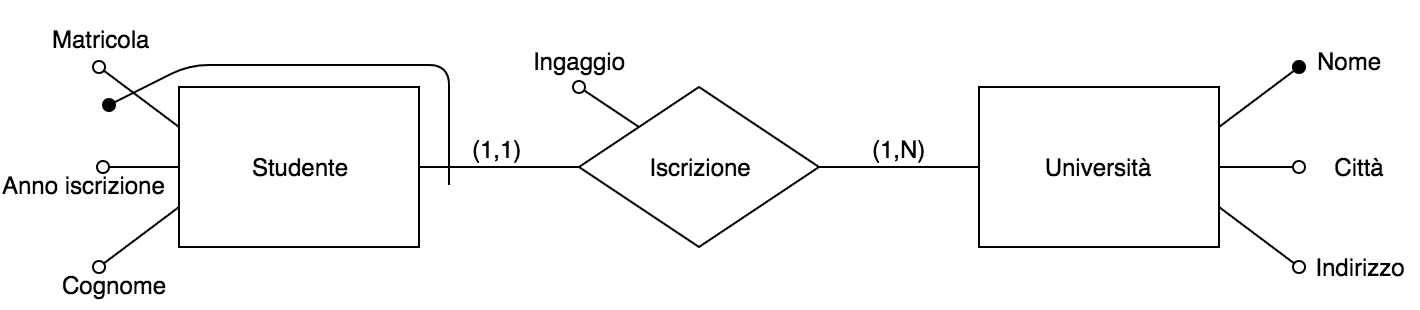
\includegraphics[scale = 0.5]{15/img9}
        \caption{Relazione con identificatore esterno}
    \end{figure}\\\\
Lo schema relazionale corrispondente a questo schema è il seguente:
    \begin{equation}\begin{aligned}
        STUDENTE(\underline{Matricola, NomeUniversita}, Cognome, AnnoIscrizione)\\
        UNIVERSITA(\underline{Nome}, Citta, Indirizzo)
    \end{aligned}\end{equation}
In questo schema relazionale esiste il vincolo d'integrità referenziale tra l'attributo $NomeUniversita$ della relazione $STUDENTE$ e l'attributo $Nome$ della relazione $UNIVERSITA$.\\\\
Come abbiamo potuto notare nell'esempio, rappresentando l'identificatore esterno si rappresenta direttamente anche l'associazione tra le due entità. Le entità identificate esternamente partecipano all'associazione sempre con una cardinalità minima e massima pari a uno.\\
Questo tipo di traduzione è valido indipendentemente dalla cardinalità con cui l'altra entità partecipa all'associazione.

\subsection{Associazioni uno a uno}
Per le associazioni uno a uno ci sono, in genere, diverse possibilità di traduzione.\\
Consideriamo il seguente schema, in cui la partecipazione di entrambe le entità è obbligatoria:
    \begin{figure}[h!]
        \centering
        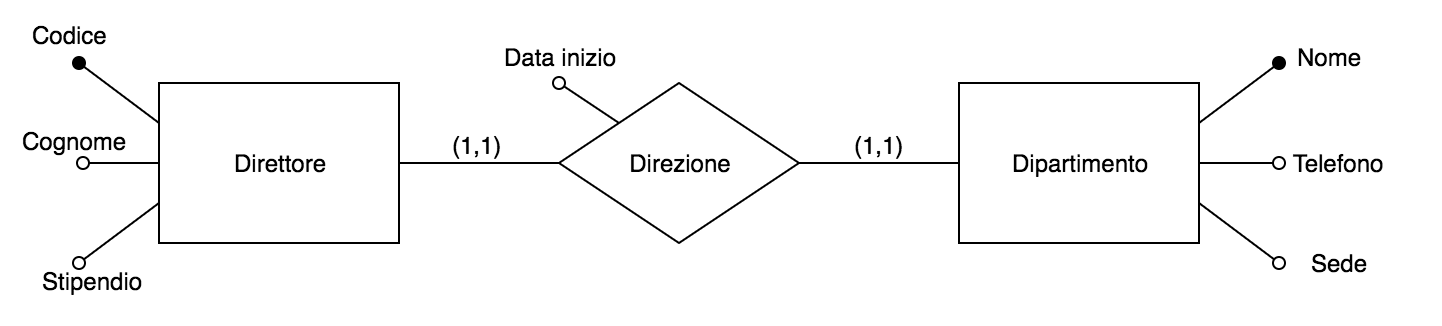
\includegraphics[scale = 0.5]{15/img10}
        \caption{Relazione uno a uno}
    \end{figure}\\\\
Un possibile schema relazionale corrispondente a questo schema è il seguente:
    \begin{equation}\begin{aligned}
        DIRETTORE(\underline{Codice}, Cognome, Stipendio, DipartimentoDiretto, InizioDirezione)\\
        DIPARTIMENTO(\underline{Nome}, Telefono, Sede)
    \end{aligned}\end{equation}
In questo schema esiste il vincolo d'integrità referenziale tra l'attributo $DipartimentoDiretto$ della relazione $DIRETTORE$ e l'attributo $Nome$ della relazione $DIPARTIMENTO$, oppure:
    \begin{equation}\begin{aligned}
        DIRETTORE(\underline{Codice}, Cognome, Stipendio)\\
        DIPARTIMENTO(\underline{Nome}, Telefono, Sede, Direttore, InizioDirezione)
    \end{aligned}\end{equation}
In questo secondo schema esiste il vincolo d'integrità referenziale tra l'attributo $Direttore$ della relazione $DIPARTIMENTO$ e l'attributo $Codice$ della relazione $DIRETTORE$.\\
È possibile, quindi, rappresentare l'associazione in una qualunque delle relazioni che rappresentano le due entità.\\\\
Trattandosi di una relazione biunivoca tra le occorrenze delle entità, sembrerebbe possibile un'ulteriore alternativa nella quale si rappresentano tutti i concetti i un'unica relazione contenente tutti gli attributi in gioco.\\
Questa alternativa è, però, da escludere perché non dobbiamo dimenticare che lo schema E-R che stiamo traducendo è il risultato di una fase di ristrutturazione nella quale sono state effettuate precise scelte anche riguardo l'accorpamento e il partizionamento di entità.\\
Questo significa che, se nello schema E-R ristrutturato abbiamo due entità collegate da una relazione uno a uno, vuol dire che abbiamo ritenuto conveniente tenere separati i due concetti ed è quindi inopportuno fonderli in sede di traduzione verso il modello relazionale.\\\\
Consideriamo ora il seguente schema, in cui soltanto un'unità ha partecipazione opzionale:
    \begin{figure}[h!]
        \centering
        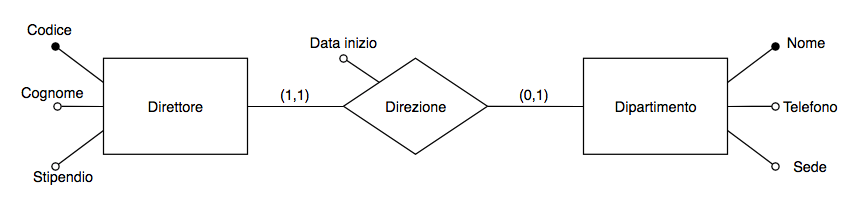
\includegraphics[scale = 0.5]{15/img10b}
        \caption{Relazione uno a uno}
    \end{figure}\\\\
In questo caso abbiamo una soluzione preferibile rispetto alle altre:
    \begin{equation}\begin{aligned}
        IMPIEGATO(\underline{Codice}, Cognome, Stipendio)\\
        DIPARTIMENTO(\underline{Nome}, Telefono, Sede, Direttore, InizioDirezione)
    \end{aligned}\end{equation}
Per lo schema ottenuto esiste il vincolo d'integrità referenziale tra l'attributo $Direttore$ della relazione $DIPARTIMENTO$ e l'attributo $Codice$ della relazione $IMPIEGATO$.\\
Questa alternativa è preferibile rispetto a quella in cui l'associazione viene rappresentata nella relazione $IMPIEGATO$ mediante il nome del dipartimento diretto perché avremmo, per questo attributo, possibili valori nulli.\\\\
Consideriamo ora il caso in cui entrambe le entità hanno partecipazione opizonale, come nel seguente schema:
    \begin{figure}[h!]
        \centering
        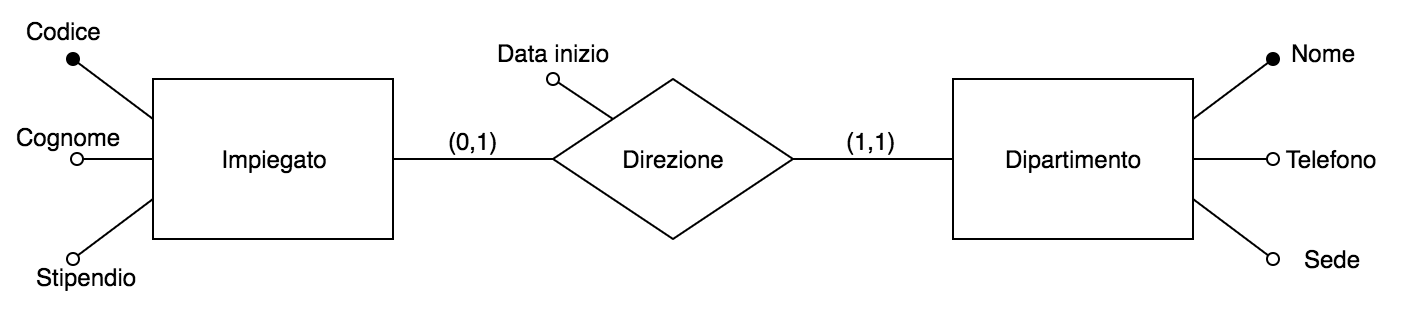
\includegraphics[scale = 0.5]{15/img11}
        \caption{Relazione uno a uno}
    \end{figure}\\\\
In questo caso abbiamo una soluzione preferibile rispetto alle altre:
    \begin{equation}\begin{aligned}
        IMPIEGATO(\underline{Codice}, Cognome, Stipendio)\\
        DIPARTIMENTO(\underline{Nome}, Telefono, Sede)\\
        DIREZIONE(\underline{Direttore}, Dipartimento, DataInizioDirezione)
    \end{aligned}\end{equation}
Su questo schema abbiamo due vincoli d'integrità referenziale: uno tra l'attributo $Direttore$ della relazione $DIREZIONE$ e l'attributo $Codice$ della relazione $IMPIEGATO$ e l'altro tra l'attributo $Dipartimento$ della relazione $DIREZIONE$ e l'attributo $Nome$ della relazione $DIPARTIMENTO$.\\
Questa soluzione ha il vantaggio, rispetto a quella in cui si accorpa la relazione $DIREZIONE$ in una delle altre due relazioni (come nel caso precedente), di non presentare mai valori nulli sugli attributi che rappresentano l'associazione. Per contro, abbiamo bisogno di una relazione in più con un conseguente aumento della complessità della base di dati.\\
Diciamo quindi che la soluzione con tre relazioni è da prendere in considerazione solo se il numero di occorrenze dell'associazione è molto basso rispetto alle occorrenze delle entità che partecipano all'associazione. In questo caso, c'è infatti il vantaggio di evitare la presenza di molti valori nulli.



\section{Documentazione di schemi logici}
Come nel caso della progettazione concettuale, il risultato della progettazione logica non è costituito solo da un semplice schema di una base di dati ma anche da una documentazione a esso associata.\\
Innanzitutto, buona parte della documentazione dello schema concettuale in ingresso alla fase di progettazione logica può essere ereditata dallo schema logico ottenuto come risultato di questa fase. In particolare, se i nomi dei concetti dello schema E-R sono stati riutilizzati per costruire lo schema relazionale, le regole aziendali precedentemente definite possono essere usate per documentare anche quest'ultimo.\\
A questa documentazione ne va aggiunta però dell'altra, in grado di descrivere i vincoli d'integrità referenziale introdotti dalla traduzione.\\\\
A tale riguardo, è possibile adottare un semplice formalismo grafico che ci permette di rappresentare sia le relazioni con i relativi attributi che i vincoli d'integrità referenziale esistenti tra le varie relazioni.\\
Un esempio di tale rappresentazione, di facile comprensione, è dato dal seguente schema:
    \begin{figure}[h!]
        \centering
        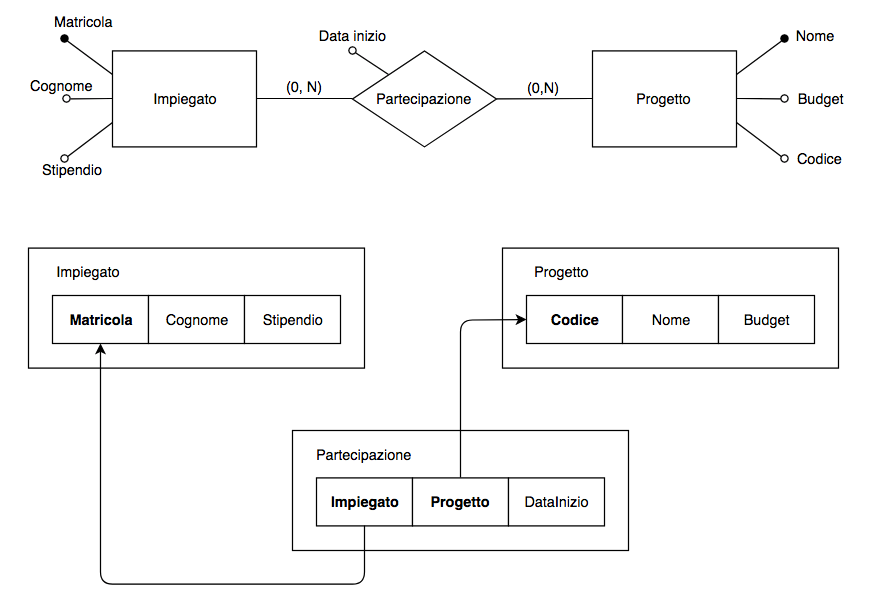
\includegraphics[scale = 0.5]{15/img12}
        \caption{Vincoli d'integrità}
    \end{figure}
In questi diagrammi le chiavi delle relazioni sono rappresentaete in grassetto, le frecce indicano vincoli d'integrità referenziale e la presenza di asterischi sui nomi di attributo indica la possibilità di avere valori nulli.\\\\
Osserviamo che, con questo formalismo, si riesce a mantenere traccia delle associazioni dello schema E-R originale. Questo può risultare utile per individuare, in maniera immediata, i \textbf{cammini di join}, ovvero le operazioni di join necessarie per riscostruire l'informazione rappresentata dalle associazioni originarie, nel caso dell'esempio, le informazioni sui progetti ai quali gli impiegati partecipano, attraverso il join tra $IMPIEGATO$, $PARTECIPAZIONE$ e $PROGETTO$.
